\documentclass[11pt]{article}
\usepackage{amsmath,amssymb,fancyhdr,url,graphicx,courier,xcolor,multicol,listings,tikz}
\usepackage[top=1in,bottom=1in,left=0.75in,right=0.75in,headheight=.75in]{geometry}
\usepackage[small,bf]{caption}
\definecolor{shadethmcolor}{rgb}{0.96,0.96,0.96}
\pagestyle{fancy}
\lhead{T.~Keller, Y.~Tan, K.~Huang, and C.~Li}
\rhead{CSCI 6360 Group Project}
\cfoot{\thepage/\pageref{LastPage}}
\frenchspacing
%%%%%%%%%%%%%%%%%%%%%%%%%%%%%%%%%%%%%%%%%%%%%%%%%%%%%%%%%%%%%%%%%%%%%%%%%%%%%%%%%%%%%%%%%%%%%%%%%%%%
\definecolor{codebg}{gray}{0.8}
\renewcommand{\headrulewidth}{0.01in} \renewcommand{\footrulewidth}{0.01in}
\newcommand{\code}[1]{\colorbox{codebg}{\texttt{\footnotesize{#1}}}}
\lstset{language=C++,basicstyle=\footnotesize\ttfamily,language=bash,backgroundcolor=\color{codebg},xleftmargin=0pt,breaklines=true,alsoletter={--,/,[,=},alsodigit={-},showstringspaces=false,breakindent=0em,prebreak={ \textbackslash},postbreak={\phantom{m}}}
\usetikzlibrary{arrows,calc,backgrounds}
\tikzstyle{na} = [rectangle,draw=black,anchor=west]
\tikzstyle{nb} = [rectangle,draw=blue,anchor=west]
\tikzstyle{nz} = [rectangle,draw=red,anchor=west]
%%%%%%%%%%%%%%%%%%%%%%%%%%%%%%%%%%%%%%%%%%%%%%%%%%%%%%%%%%%%%%%%%%%%%%%%%%%%%%%%%%%%%%%%%%%%%%%%%%%%
\begin{document}
\centerline{\LARGE{\bfseries MMSP Compute and I/O Performance on AMOS}}
\begin{multicols}{4}\centering
 \textbf{Trevor Keller}\\
 \emph{Materials Science}
 
 \textbf{Yixuan Tan}\\
 \emph{Mechanical Engineering}

 \textbf{Kun Huang}\\
 \emph{Physics}
 
 \textbf{Congrui Li}\\
 \emph{Computer Science}

\end{multicols}

\begin{center}
\texttt{\{kellet,tany3,huangk4,lic10\}@rpi.edu}

\vskip\baselineskip
Rensselaer Polytechnic Institute\\110 Eighth Street\\Troy, NY 12180

\vskip\baselineskip
May 8, 2014
\end{center}


\begin{abstract}
\noindent Parallel computing is a key capability for numerical models of physical systems.
Our group is interested specifically in the problem of grain growth in 3-dimensional polycrystalline metals.
Using the knowledge we gained in CSCI-6360, we have upgraded an existing research code, the Mesoscale Microstructure Simulation Project (MMSP), to use pthreads for computational performance gains and MPI-IO for parallel output of checkpoint files.
We discuss the speedup and bandwidth results, with recommendations for the ``best'' simulation conditions.

Our code is available online via \url{https://github.com/fifthblackbird/PPCproject}, and will be integrated into MMSP in the near future.
\end{abstract}

\begin{multicols*}{2}
\section{Introduction}
The Mesoscale Microstructure Simulation Project (MMSP) is a C++ code for parallel simulation of physical systems using Monte Carlo, phase-field, and similar methods.\footnote{\url{http://matforge.org/mmsp} and \url{http://github.com/mesoscale/mmsp}}
MMSP implements a 3-dimensional grid class, with back-end support for parallel synchronization and file I/O using MPI.
This grid facilitates computation of spatial derivatives by exchanging ``ghost'' cells between spatially adjacent ranks:
essentially, each face of the local 3-D grid needs to be sent to the MPI rank sharing that face.
This is a common feature of codes for numerical integration of partial differential equations;
indeed, while designed for materials science, MMSP could be applicable to a large number of numerical computing tasks.

To date, MMSP has been tested and used extensively on workstation-class machines, occasionally on clusters (such as the CCI Opteron cluster), and almost never on supercomputers.
Past efforts at MPI-IO have used \texttt{MPI\_File\_iwrite\_shared} and \texttt{MPI\_File\_iwrite\_at}, with default (\texttt{MPI\_NULL}) hints.
The code had not previously taken the underlying filesystem into consideration.
On AMOS, the GPFS has a blocksize of 8MB, while the MPI ranks may only write a few KB each.
This produced contention for a common GPFS block between thousands of processors and, ultimately, failure to write anything at all.
We chose to address this problem by implementing an explicit two-stage accumulate-and-write output function, wherein a few MPI ranks gather data from the upstream ranks that would contend for the same block;
only the accumulator ranks write to disk, once their output buffers are full.


\section{Algorithms}
We selected two strong-scaling grain growth models -- Potts Monte Carlo and phase-field -- for comparison.

\subsection*{Voronoi Tessellation}
3-D simulations need a starting point, and the Poisson-Voronoi tessellation is the most common for grain growth simulations.
These tessellations are the combination of a Poisson point process for generating random seed points, followed by the Voronoi tessellation of space around those seeds;
that is to say, any point in space closer to one seed than any other belongs to that seed's domain.
This is done using the algorithm in Listing~\ref{lst:voro}, for a mesh containing $N$ nodes; it is a na\"ive algorithm, but easy to parallelize.
Since the Voronoi tessellation is embarassingly parallel, we chose not to devote resources to improving this implementation.
We did, however, modify the reference algorithm in the following ways:
\begin{enumerate}
 \item Instead of an \texttt{MPI\_Allgather} over every MPI rank, we determined which ranks were adjacent along a domain face or through a domain corner, and retrieved seeds from those ranks, only.
 \item We implemented pthreads by subdividing the loop \code{for (n=0; n<N; n++)} among the available threads, \code{for (n=nlo; n<nhi; n++)} with \texttt{nlo}$\geq0$ and \texttt{nhi<N} defined for each thread.
 \item Instead of the built-in random number generator, we generate seeds with the Mersenne twister.
\end{enumerate}
This reduced the runtime from $\mathcal{O}(2\ \mathrm{hours})$ to under a minute.
The final result of a Voronoi tessellation in 2-D ($1024^2$ mesh) performed on AMOS is provided in Fig.~\ref{fig:voro}.

\begin{center}\begin{minipage}{0.45\textwidth}\centering
  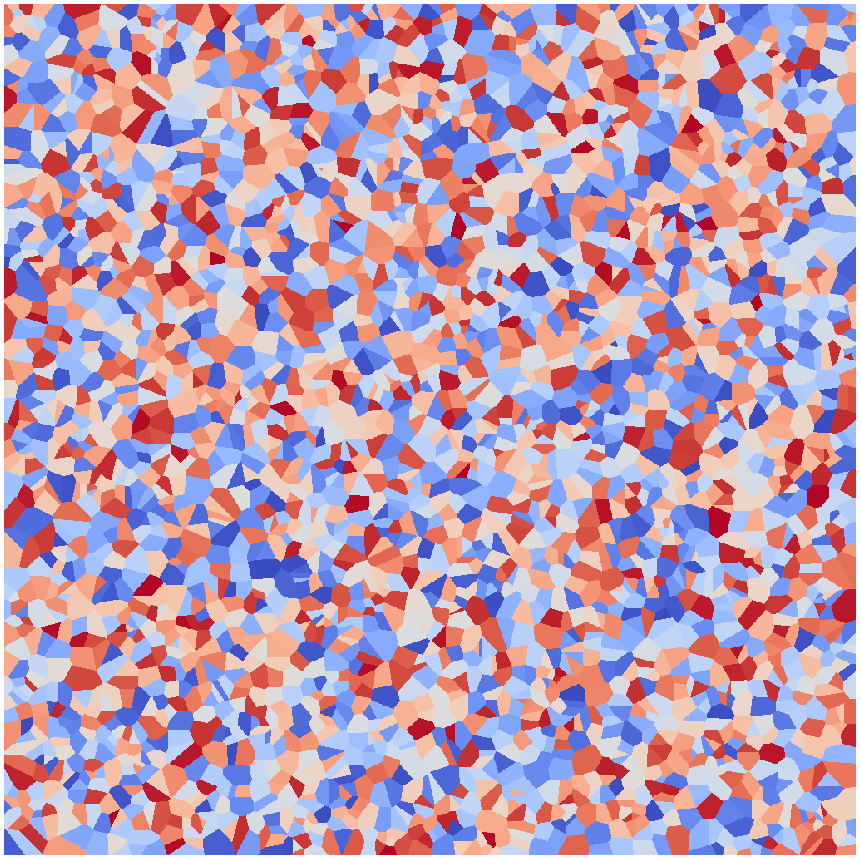
\includegraphics[width=\textwidth]{voronoi}
  \captionof{figure}{Voronoi tessellation produced by our code on AMOS ($1024\times1024$ mesh, $3336$ seeds; $1024$ threads). Runtime: 0.07 sec. Note the straight edges.\label{fig:voro}}
\end{minipage}\end{center}


\begin{minipage}{0.45\textwidth}
\begin{center}
\begin{lstlisting}
#include<cmath>
typedef struct {
  int x; int y; int z;
} int3;
void PVT(MMSP::grid& grid, int nseeds=10000)
{
  int np = MPI::COMM_WORLD.Get_size();
  while (nseeds%np != 0) ++nseeds;
  int S = nseeds/np;
  int3* seeds = new int3[S];
  int3* all_seeds = new int3[nseeds];
  for (i=0; i<nseeds; i++) {
    seeds[i].x=rand()%grid.xlength();
    seeds[i].y=rand()%grid.ylength();
    seeds[i].z=rand()%grid.zlength();
  }
  S *= 3;
  nseeds *= 3; 
  MPI_Allgather(seeds, S, MPI_INT, all_seeds, nseeds, MPI_INT, MPI_Comm_World);
  S /= 3;
  nseeds /= 3;
  for (n=0; n<N; n++) {
    int3 pos = MMSP::position(grid, n);
    int best;
    double min = std::pow(domain_size, 2);
    for (i=0; i<nseeds; i++) {
      dist = std::sqrt(std::pow(pos.x - seeds[i].x, 2) + std::pow(pos.y - seeds[i].y, 2) + std::pow(pos.z - seeds[i].z, 2))
      if (dist<min) {
	best = i;
	min=dist;
      }
    }
    grid(n) = best;
  }
  delete [] seeds;
  delete [] all_seeds;
}
\end{lstlisting}
\captionof{lstlisting}{Na\"ive Poisson-Voronoi tessellation algorithm.\label{lst:voro}}
\end{center}
\vskip\baselineskip
\end{minipage}

\subsection*{Potts Monte Carlo Model}
The overall grid is portioned in to different local grids so that each processor is assigned a contiguous subgrid.
In two dimensions this is a small rectangular section, and in three dimensions it is a rectangular box.
Each processor also stores a copy of the narrow strips (or planes in three dimensions) of lattice sites that immediately adjoin its sub-domain and which are actually owned by neighboring processors.
This allows a processor to check neighboring spin values of sites on the edge of its sub-domain.
With these data structures, every processor can now simultaneously flip spins in its sub-domain without violating the rule of detailed balance, 
so long as one processor does not choose a lattice site on an edge of its sub-domain at the same time the processor adjoining that edge does likewise.
We enforce this restriction in our parallel Potts algorithm by ``slicing'' the subgrid as shown in Figure 1. 
lattice site is represented by a square (not the corners of the square) and assigned a ``sublattice'' number, 0 or 1.

A subgrid is divided into sublattices as in Figure 1, where only the lattice sites assigned to sublattice-0 are now shown as shaded.
The key point is that the 2 neighbors of a sublattice-0 lattice site do not include any other sublattice-0 lattice sites.
The parallel Monte Carlo Potts grain growth algorithm for one sweep can now be written as follows:

\begin{minipage}{0.475\textwidth}
\begin{center}
\begin{lstlisting}
Loop over sublattice (i)
  Loop over all lattice sites of sublattice i within my subgrid
    Pick a new spin value randomly.
    Compute the energy change for the site to change to the new spin.
    Accept or reject the change based on the Boltzmann criterion.
  End lattice site loop
  Exchange sites along edge of my subgrid with neighboring processors to acquire current neighbor spin values.
End color loop
\end{lstlisting}
\captionof{lstlisting}{Monte Carlo algorithm.\label{lst:mc}}
\end{center}
\vskip\baselineskip
\end{minipage}

This algorithm works for both 2-D and 3-D lattices. Also, the communication of subgrid ``edges'' becomes ``planes'' in 3-D. 


\begin{center}
\begin{minipage}{0.475\textwidth}\centering
  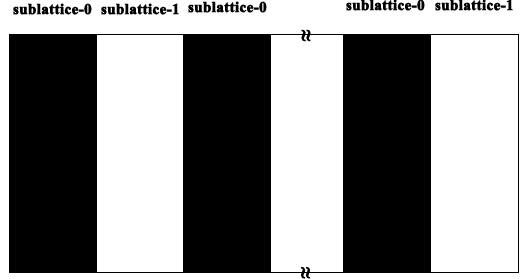
\includegraphics[width=\textwidth]{mc-fig-01}
  \captionof{figure}{Slicing subgrid into sublattice used for parallel Potts grain growth algorithm.\label{fig:mc1}}
\end{minipage}

\begin{minipage}{0.475\textwidth}\centering
  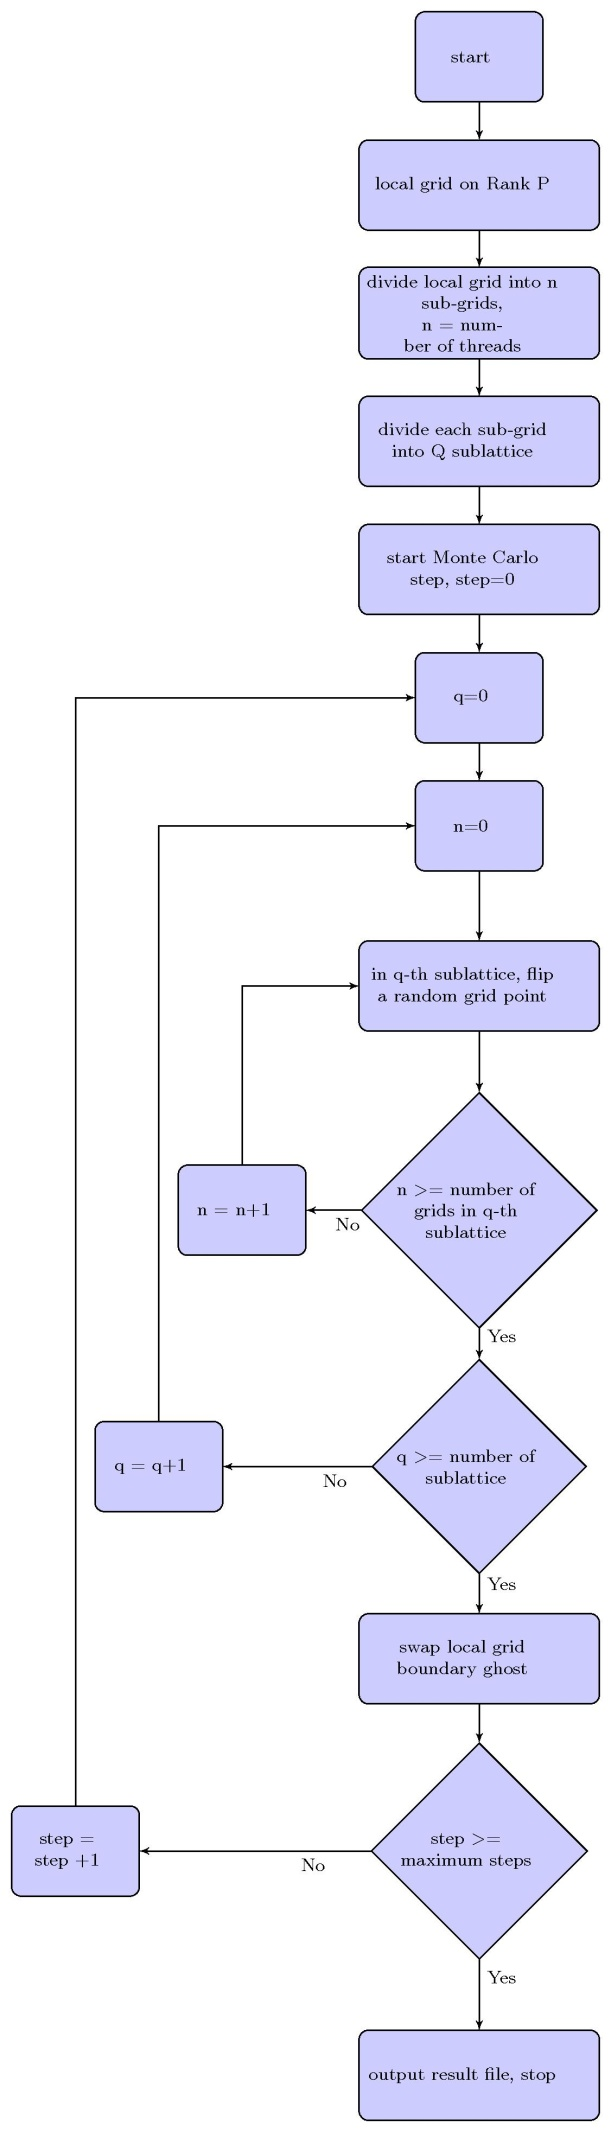
\includegraphics[height=6.5in]{mc-fig-02}
  \captionof{figure}{\emph{No caption provided.}\label{fig:mc2}}
\end{minipage}
\end{center}

An example of 2-D grain growth using the Potts Monte Carlo physical model is given in Fig.~\ref{fig:voroggmc}.

\begin{center}\begin{minipage}{0.45\textwidth}\centering
  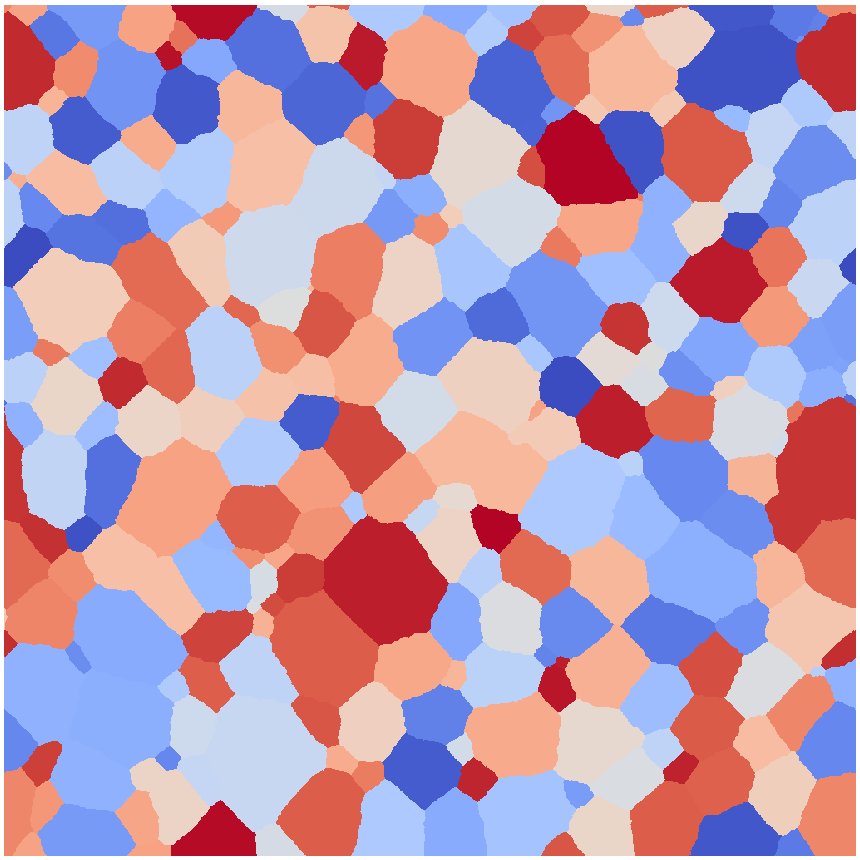
\includegraphics[width=\textwidth]{graingrowth-mc}
  \captionof{figure}{Grain growth produced by our phase-field code on AMOS ($5000$ iterations, $1024$ threads). Runtime: 18 minutes. Note the curved edges.\label{fig:voroggmc}}
\end{minipage}\end{center}


\subsection*{Phase-Field Model}
Phase-field models are useful for mesoscale simulations of cellular materials:
the models have a characteristic length scale $\mathcal{O}(1\ \mu\mathrm{m})$, with ``cells'' distinguished by some characteristic such as solid fraction (instead of liquid), magnetic field alignment, or grain orientation.
The interfaces between adjacent cells are modeled through the smooth, continuous transition of an order parameter $\phi$ between one (existence) and zero (absence).
The model implemented for this project assigns one order parameter to each grain, and each node in the computational mesh contains a sparse vector $\{\phi\}$, ranging in size between one and 27 entries (in 3-D) \cite{Steinbach1999}.
Grain growth in these simulations occurs by numerically integrating the parabolic partial differential equation-of-motion,
\begin{align}
\frac{\partial\phi_i}{\partial t} = -\frac{\mu}{S}\sum\limits_{j\neq i}^S\Bigg[
  &\sum\limits_{k\neq i}^S\bigg(\frac{1}{2}\varepsilon^2\nabla^2\phi_k+\omega|\phi_k|\bigg)\notag\\
  -&\sum\limits_{\ell\neq j}^S\bigg(\frac{1}{2}\varepsilon^2\nabla^2\phi_\ell+\omega|\phi_\ell|\bigg)\Bigg],\label{eqn:pf}
\end{align}
using information from the $S$-dimensional sparse vector $\{\phi\}$ at each point, with interfacial mobility $\mu$ and model parameters $\varepsilon$ and $\omega$.
The Laplacian operator $\nabla^2 = \frac{\partial^2}{\partial x^2} + \frac{\partial^2}{\partial y^2} + \frac{\partial^2}{\partial z^2}$;
in each dimension, the Laplacian operator for a given order parameter is
\begin{equation}
\frac{\partial^2\phi}{\partial x^2} \approx \frac{\Delta(\Delta\phi)}{\Delta x^2} = \frac{\phi_{i+1} - 2\phi_i + \phi_{i-1}}{2\Delta x^2},\label{eqn:laplacian}
\end{equation}

where the values $\phi_{i+1}$ and $\phi_{i-1}$ are read from the two neighbors of point $i$. 
These second-order spatial derivatives are the reason this is not an embarassingly parallel algorithm.
At the boundary of the grid stored on each MPI rank, values of $\phi\in S$ must be set in \emph{ghost cells} with data retrieved from the adjacent grid.
The more MPI ranks, the more ghost data, and the higher the network load.
This intercommunication of boundary values occurs after each numerical integration iteration; that is to say, the serial computation and parallel data synchronization occur at different times.
Listing~\ref{lst:pf} summarizes the phase-field algorithm as-implemented for $T$ timesteps on a local grid containing $N$ nodes, using only one thread per MPI rank.
\begin{minipage}{0.475\textwidth}
\begin{center}
\begin{lstlisting}
void initialize(MMSP::grid);
MMSP::sparse update(MMSP::grid, int);
void ghostswap(MMSP::grid);
void swap(MMSP::grid, MMSP::grid);

int main()
{
  MMSP::grid pfgrid;
  MMSP::grid newgrid;
  PVT(pfgrid);
  for (t=0; t<T; t++) {
    ghostswap(pfgrid);
    for (n=0; n<N; n++)
      newgrid(n) = update(pfgrid, n);
    swap(pfgrid, newgrid);
  }
  return 0;
}
\end{lstlisting}
\captionof{lstlisting}{Phase-field algorithm. \texttt{PVT()} was given in Listing~\ref{lst:voro}; \texttt{update()} implements Eqn.~\ref{eqn:pf}.\label{lst:pf}}
\end{center}
\vskip\baselineskip
\end{minipage}

The independence of computation from communication and the increasing communication overhead associated with adding MPI ranks makes pthreading a favorable approach for maximizing performance in this model.
To use pthreads, Listing~\ref{lst:pf} is modified simply to loop over \code{n=nlo; n<nhi; n++}, with \texttt{nlo}$\geq0$ and \texttt{nhi}$<$\texttt{N} defined for each pthread.

An example of 2-D grain growth using the phase-field physical model is given in Fig.~\ref{fig:vorogg}.

\begin{center}\begin{minipage}{0.45\textwidth}\centering
  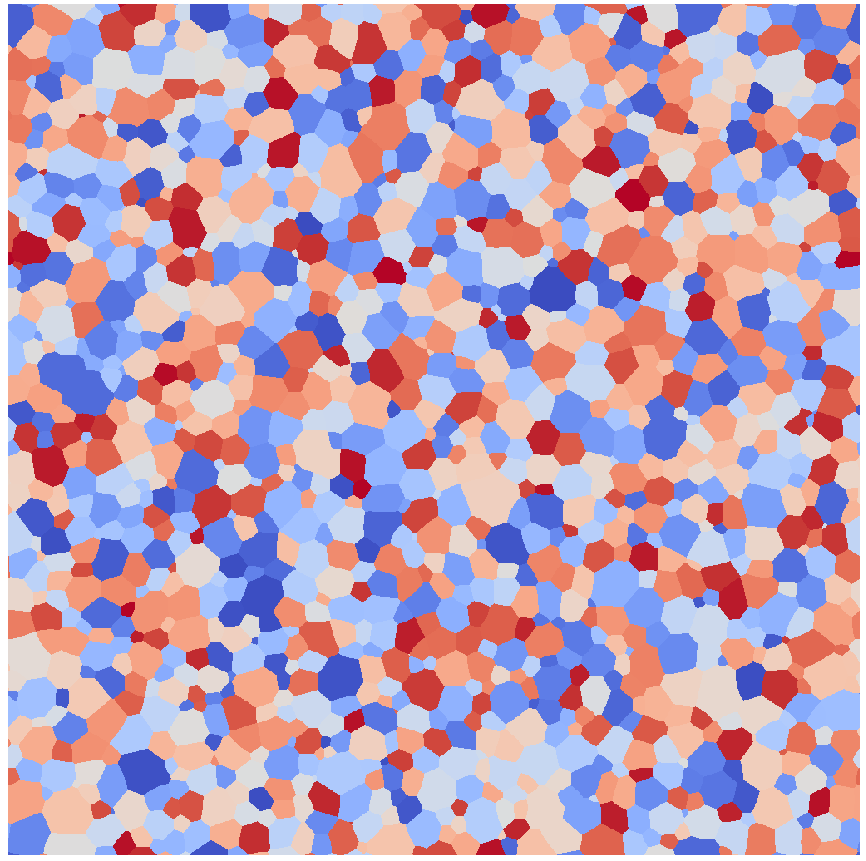
\includegraphics[width=\textwidth]{graingrowth}
  \captionof{figure}{Grain growth produced by our phase-field code on AMOS ($5000$ iterations, $1024$ threads). Runtime: 13 minutes. Note the curved edges, and smaller grains than the Potts MC model.\label{fig:vorogg}}
\end{minipage}\end{center}

\subsection*{Two-Step I/O}
The stock MMSP distribution comes with an \texttt{output} function which synchronizes data sizes across all MPI ranks, sets a local offset, then calls \texttt{MPI\_File\_iwrite\_at} with a matching \texttt{MPI\_Wait}.
The function works nicely for relatively small problems:
on the CCI Opteron cluster, grids of $400^3$ nodes wrote to disk on up to $192$ MPI ranks.
However, the stock function has never worked on our Blue Gene systems:
neither the Blue Gene/P nor AMOS ever wrote a complete MMSP file to disk.
In the rare case when the file had non-zero size, it was too small by an integer multiple of the size-per-rank expected:
some ranks were simply barred from contributing to the file.
For reference, the MMSP file structure is presented in Fig.~\ref{fig:file}.
\begin{minipage}{0.475\textwidth}
\begin{center}
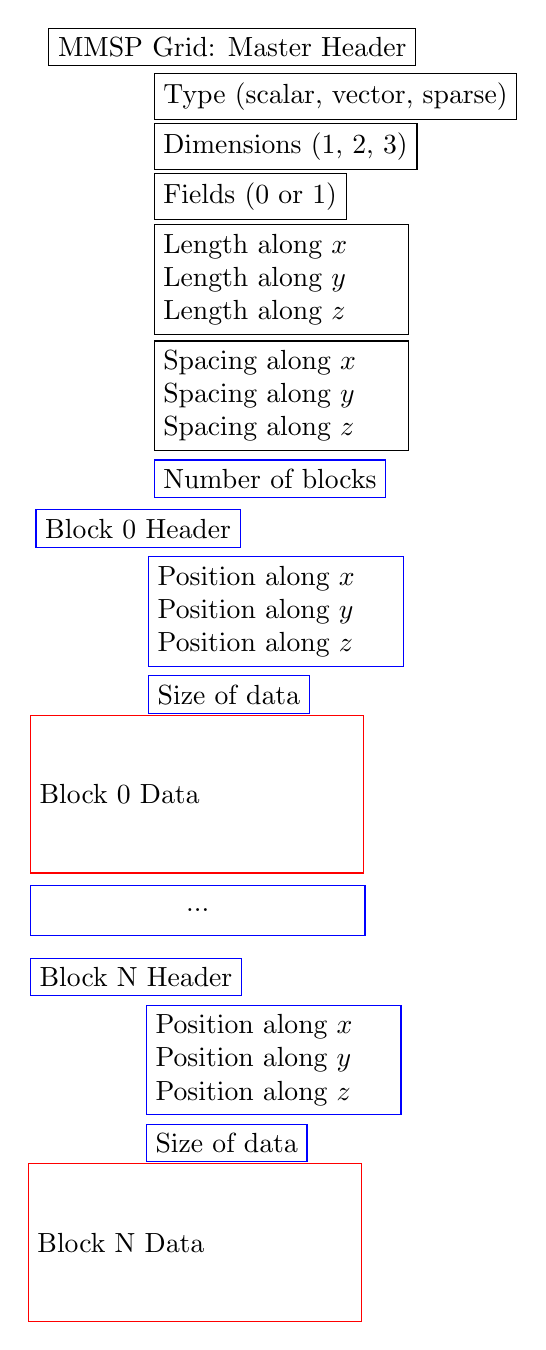
\begin{tikzpicture}[scale=0.5]
  \node[na](gh){MMSP Grid: Master Header};
  \node[na] at ($(gh)+(-2,-3\baselineskip)$) {Type (scalar, vector, sparse)};
  \node[na] at ($(gh)+(-2,-6\baselineskip)$) {Dimensions (1, 2, 3)};
  \node[na] at ($(gh)+(-2,-9\baselineskip)$) {Fields (0 or 1)};
  \node[na,text width=3cm] at ($(gh)+(-2,-14\baselineskip)$) {Length along $x$ Length along $y$ Length along $z$};
  \node[na,text width=3cm] at ($(gh)+(-2,-21\baselineskip)$) {Spacing along $x$ Spacing along $y$ Spacing along $z$};
  \node[nb] at ($(gh)+(-2,-26\baselineskip)$) {Number of blocks};
  \node[nb](sh) at ($(gh)+(-5,-29\baselineskip)$) {Block 0 Header};
  \node[nb,text width=3cm] at ($(sh)+(0.25,-5\baselineskip)$) {Position along $x$ Position along $y$ Position along $z$};
  \node[nb] at ($(sh)+(0.25,-10\baselineskip)$) {Size of data};
  \node[nz,minimum height=2cm,text width=4cm] at ($(sh)+(-2.75,-16\baselineskip)$) {Block 0 Data};
  \node[nb,minimum height=1.5\baselineskip,minimum width=4.25cm] at ($(sh)+(-2.75,-23\baselineskip)$) {...};
  \node[nb](sn) at ($(sh)+(-2.75,-27\baselineskip)$) {Block N Header};
  \node[nb,text width=3cm] at ($(sn)+(0.25,-5\baselineskip)$) {Position along $x$ Position along $y$ Position along $z$};
  \node[nb] at ($(sn)+(0.25,-10\baselineskip)$) {Size of data};
  \node[nz,minimum height=2cm,text width=4cm] at ($(sn)+(-2.75,-16\baselineskip)$) {Block N Data};
\end{tikzpicture}
\captionof{figure}{MMSP file format. Fields surrounded by black boxes are ASCII, blue are binary, red are \texttt{zlib}-compressed binary.\label{fig:file}}
\end{center}
\vskip\baselineskip
\end{minipage}


Since the MMSP grid can grow fairly large, \texttt{zlib} compression is used on-the-fly;
filesizes range between $10$ MB for the initial condition to $3$ GB for intermediate stages of grain growth.
Our working hypothesis for AMOS's failure to write is that dividing the smaller files among thousands of processors created extreme contention for common blocks on the parallel filesystem, or else multiple GPFS servers attempted to allocate space for the same block.




\section{Results}


\section{Analysis}


\section{Conclusions}


\section{Contributions}
\begin{itemize}
 \item Kun Huang\\
	MC algorithm implementation and pthreading
 \item Trevor Keller\\
	Voronoi algorithm selection and implementation; parallel PF selection and implementation; MPI-IO algorithm design and implementation
 \item Congrui Li\\
	pthread PF and Voronoi
 \item Yixuan Tan\\
	MC algorithm selection and implementation
\end{itemize}

\label{LastPage}
\begin{footnotesize}
\begin{thebibliography}{1}
  \bibitem{Steinbach1999} I.~Steinbach and F.~Pezzolla. ``A generalized field method for multiphase transformations using interface fields.'' \emph{Physica D: Nonlinear Phenomena} \textbf{134} (1999) 385--393.
\end{thebibliography}
\end{footnotesize}
\end{multicols*}
\end{document}
